\chapter{Data acquisition for CHIPS} %%%%%%%%%%%%%%%%%%%%%%%%%%%%%%%%%%%%%%%%%%%%%%%%%%%%%%%%%%%%%
\label{chap:daq} %%%%%%%%%%%%%%%%%%%%%%%%%%%%%%%%%%%%%%%%%%%%%%%%%%%%%%%%%%%%%%%%%%%%%%%%%%%%%%%%%

\begin{comment} % PLAN %%%%%%%%%%%%%%%%%%%%%%%%%%%%%%%%%%%%%%%%%%%%%%%%%%%%%%%%%%%%%%%%%%%%%%%%%%%
- What makes this implementation special
- Limited resource, but brilliant capabilities
- Use existing software when possible

- Need to talk about what is novel, new and exciting!
- Not so much about the hardcore electronics details, more high level
- FINITE STATE MACHINE!!!

HARDWARE
- The White Rabbit timing system
- Km3NET hardware
- Madison hardware (novel)
- Combined systems

SOFTWARE
- The beam spill
- Hit acquisition and handling
- Detector and data quality monitoring
\end{comment}

- Needs to able to cope with 4 degrees at bottom!
- R6091 PMTs use a Cockroft-Walton board that generates a positive voltage, to hold the anode at a
positive charged and keep the cathode grounded. This is done as the PMTs make direct contact with
the water within the detector volume which can attract electrons within the PMT to the glass
causing glass scintillation and significant noise.
- Talk about expected data through put, what we can cope with
- Jumbo frames etc

\section{The White Rabbit timing system} %%%%%%%%%%%%%%%%%%%%%%%%%%%%%%%%%%%%%%%%%%%%%%%%%%%%%%
\label{sec:daq_timing} %%%%%%%%%%%%%%%%%%%%%%%%%%%%%%%%%%%%%%%%%%%%%%%%%%%%%%%%%%%%%%%%%%%%%%

- WHite-rabbit ref in~\cite{lipinski2011}

\begin{figure} % WHITE-RABBIT COMPONENTS DIAGRAM %
    \centering
    \subcaptionbox{White Rabbit switch\label{fig:nikhef_pmt}}{%
        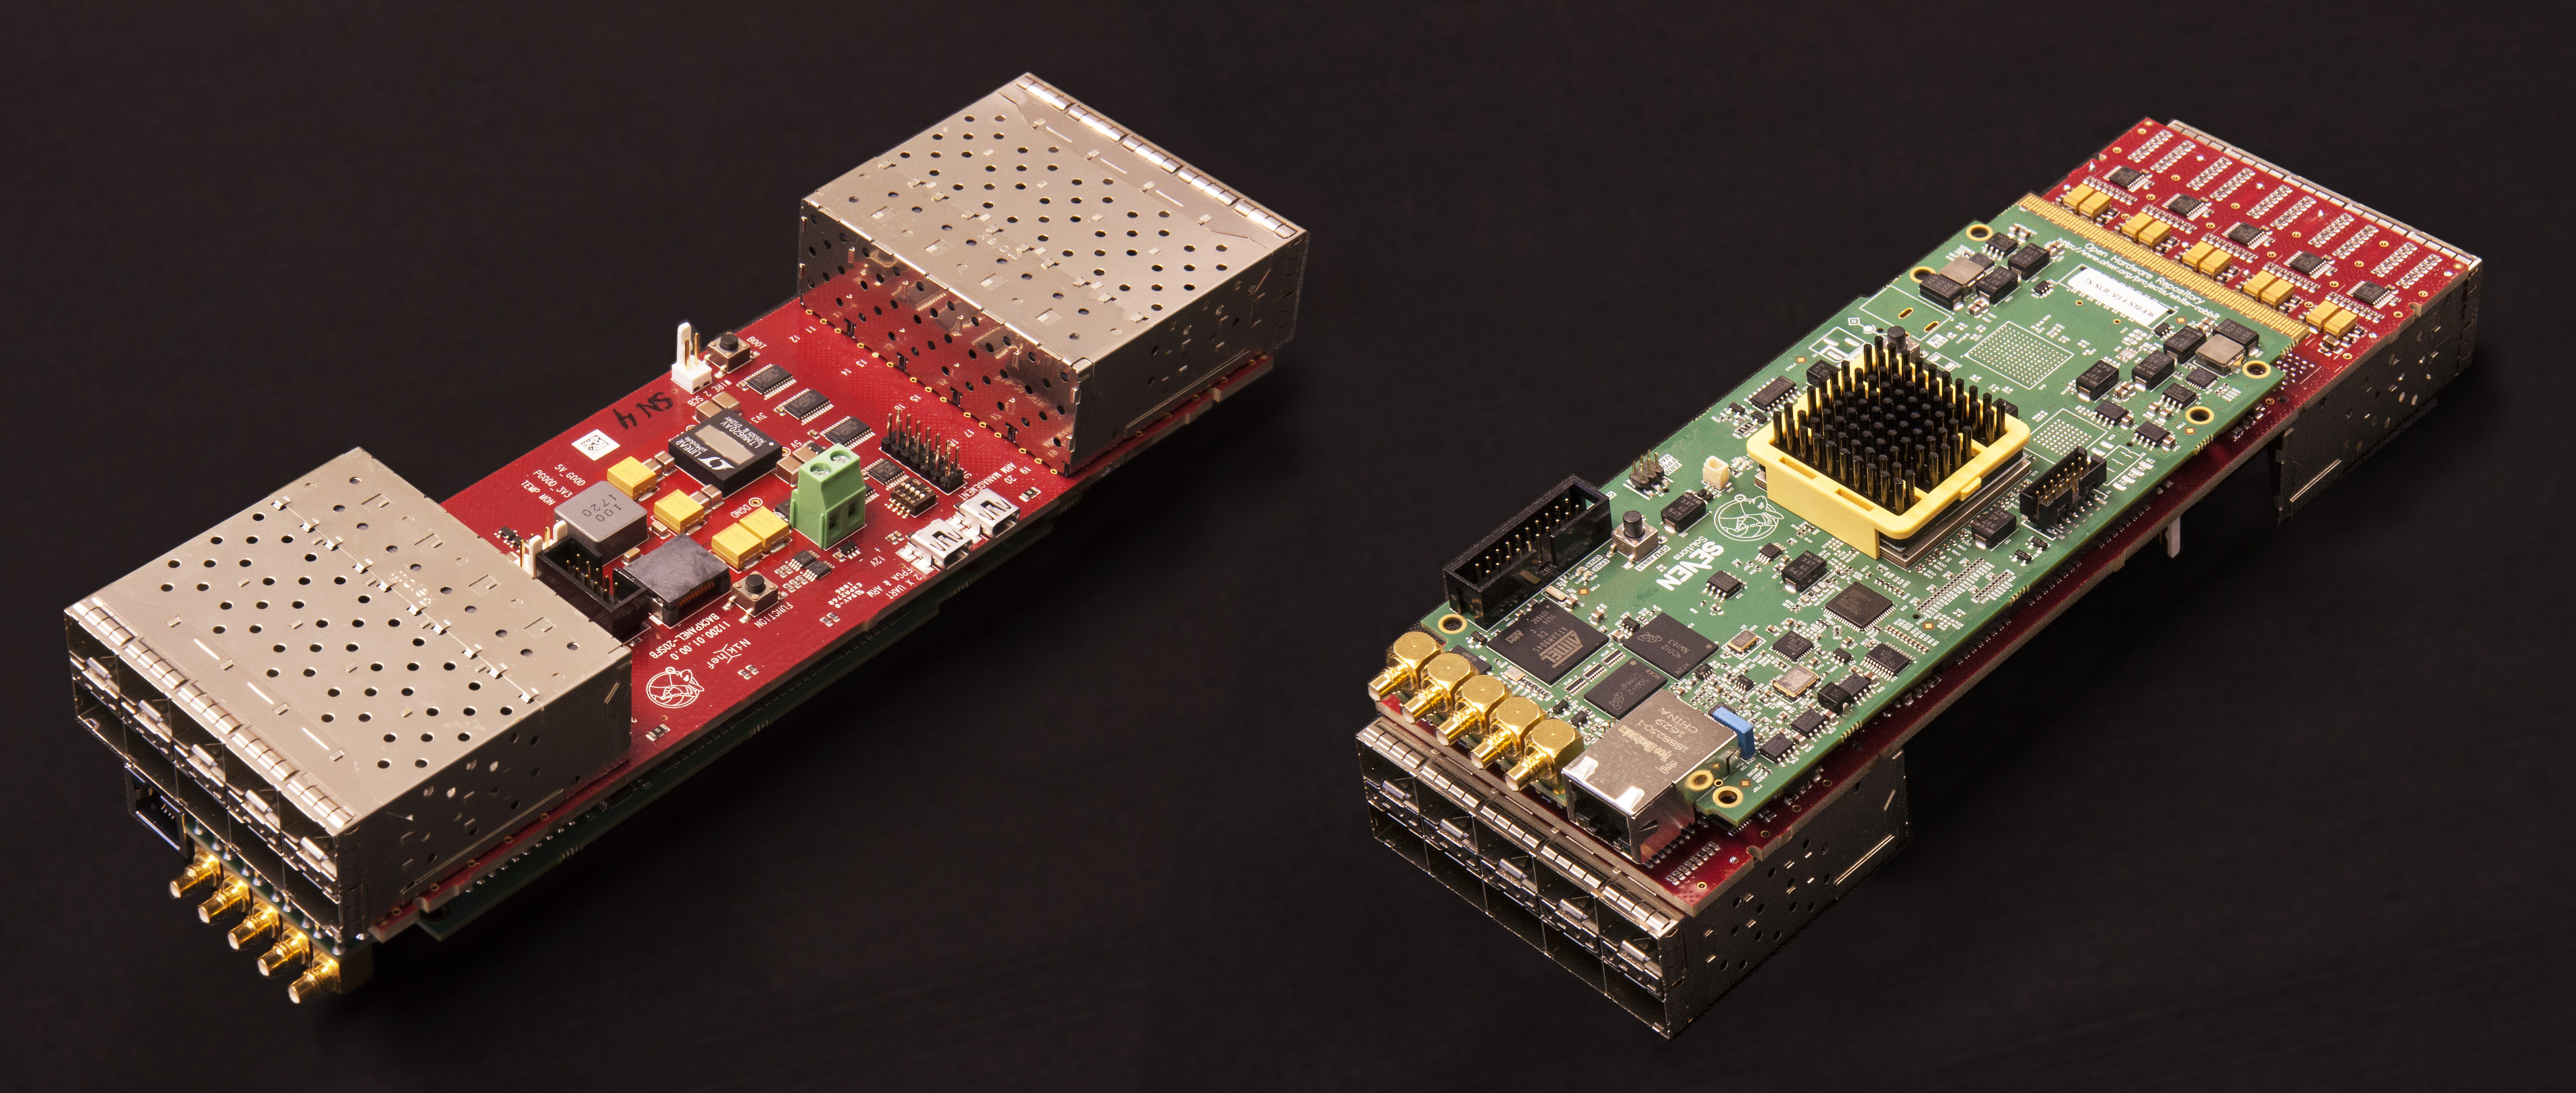
\includegraphics[height=6cm]{diagrams/5-daq/wr_switch.jpg}%
    }
    \quad
    \subcaptionbox{White Rabbit LEN\label{fig:clb}}{%
        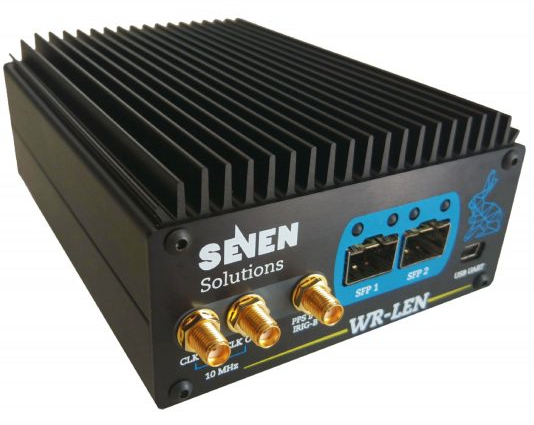
\includegraphics[height=6cm]{diagrams/5-daq/wr_len.jpg}%
    }
    \caption[Pictures of the White Rabbit timing hardware used within \chipsfive.]
    {Pictures of the White Rabbit timing hardware used within \chipsfive. A \emph{backplane-20SFP}
        version of a White rabbit switch, specially designed for \chips and KM3NeT is shown in
        (a), while the White Rabbit Lite Embedded Node (LEN) from Seven Solutions is shown in
        (b).}
\end{figure}

\begin{figure} % WHITE-RABBIT SYNC DIAGRAM %
    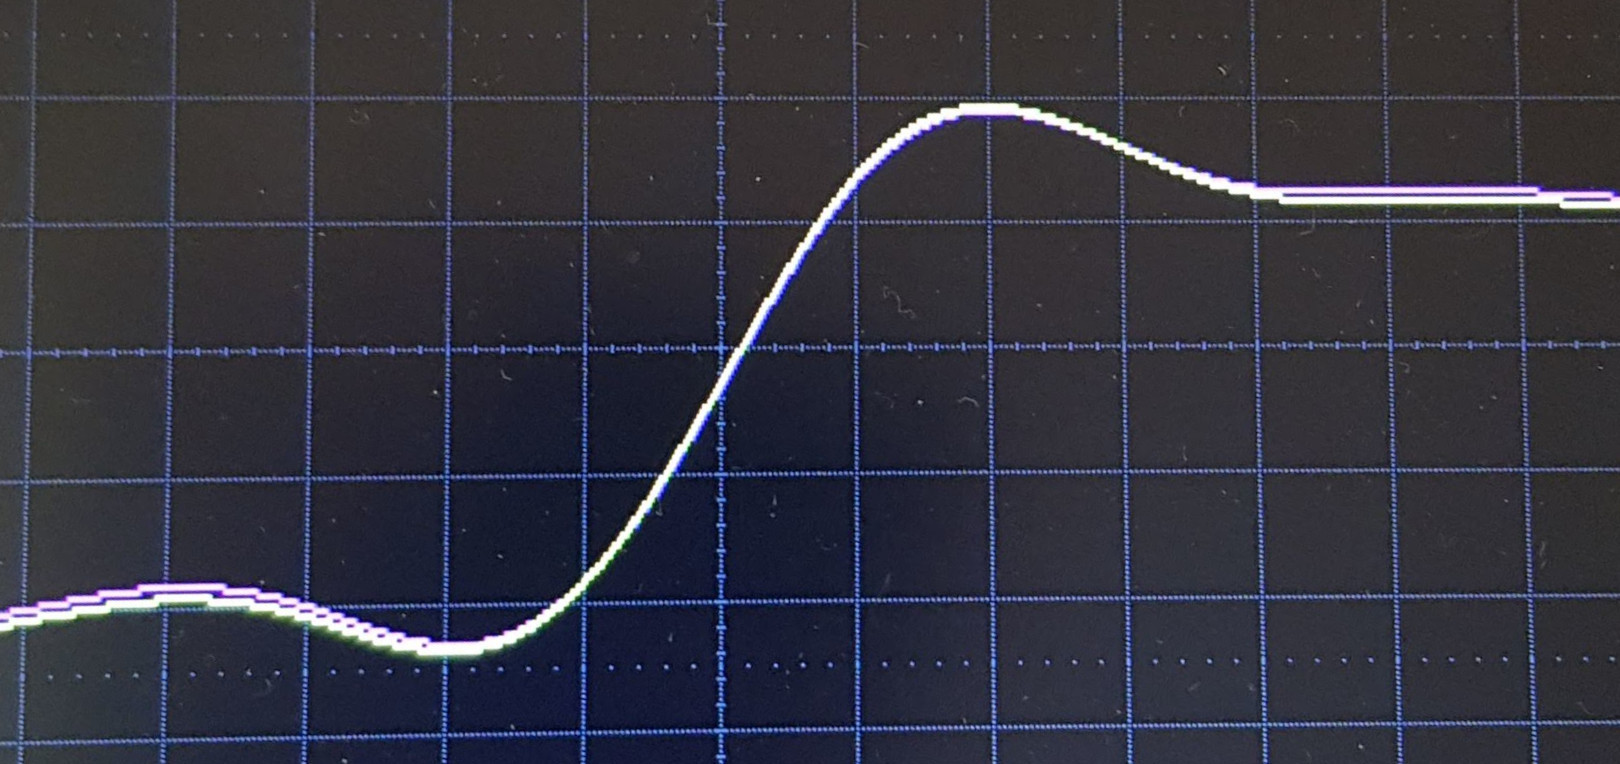
\includegraphics[width=0.8\textwidth]{diagrams/5-daq/sync.jpg}
    \caption[Picture of White Rabbit timing synchronisation seen in \chips.]
    {Picture of of oscilloscope measuring the \unit{10}{\mathrm{MHz}} White Rabbit signal of two
        switches shown in pink and yellow at either end of a \unit{500}{\mathrm{m}} long fibre.
        The vertical ticks are in nanoseconds showing the sub-nanosecond synchronisation possible
        with the White Rabbit timing system}
    \label{fig:sync}
\end{figure}

\section{Hardware} %%%%%%%%%%%%%%%%%%%%%%%%%%%%%%%%%%%%%%%%%%%%%%%%%%%%%%%%%%%%%%%%%%%%%%%%%%%%%%%
\label{sec:daq_hard} %%%%%%%%%%%%%%%%%%%%%%%%%%%%%%%%%%%%%%%%%%%%%%%%%%%%%%%%%%%%%%%%%%%%%%%%%%%%%

- Start from the bottom and work our way up!
- The task is to take TOT recorded hits, that are timestamped using the white-rabbit stuff and get
them to storage at Fermilab, all sorted, without losses, in a timely manner.
- Talk about general time resolution of the PMTs etc in the context of the overall time resolution
with the white rabbit.

\begin{figure} % TOT DIAGRAM DIAGRAM %
    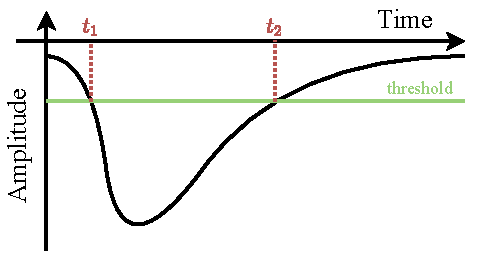
\includegraphics[width=0.7\textwidth]{diagrams/5-daq/tot.pdf}
    \caption[Illustrative diagram showing how time-over-threshold is measured.]
    {Illustrative diagram showing how time-over-threshold is measured. As soon as the rising edge
        of the charge pulse from a photon cascade passes a threshold a time is recorded, when the
        falling edge passes the threshold again a second time is recorded. The difference in time
        is output by the electronics as the time-over-threshold value.}
    \label{fig:tot}
\end{figure}

\begin{figure} % DAQ DIAGRAM %
    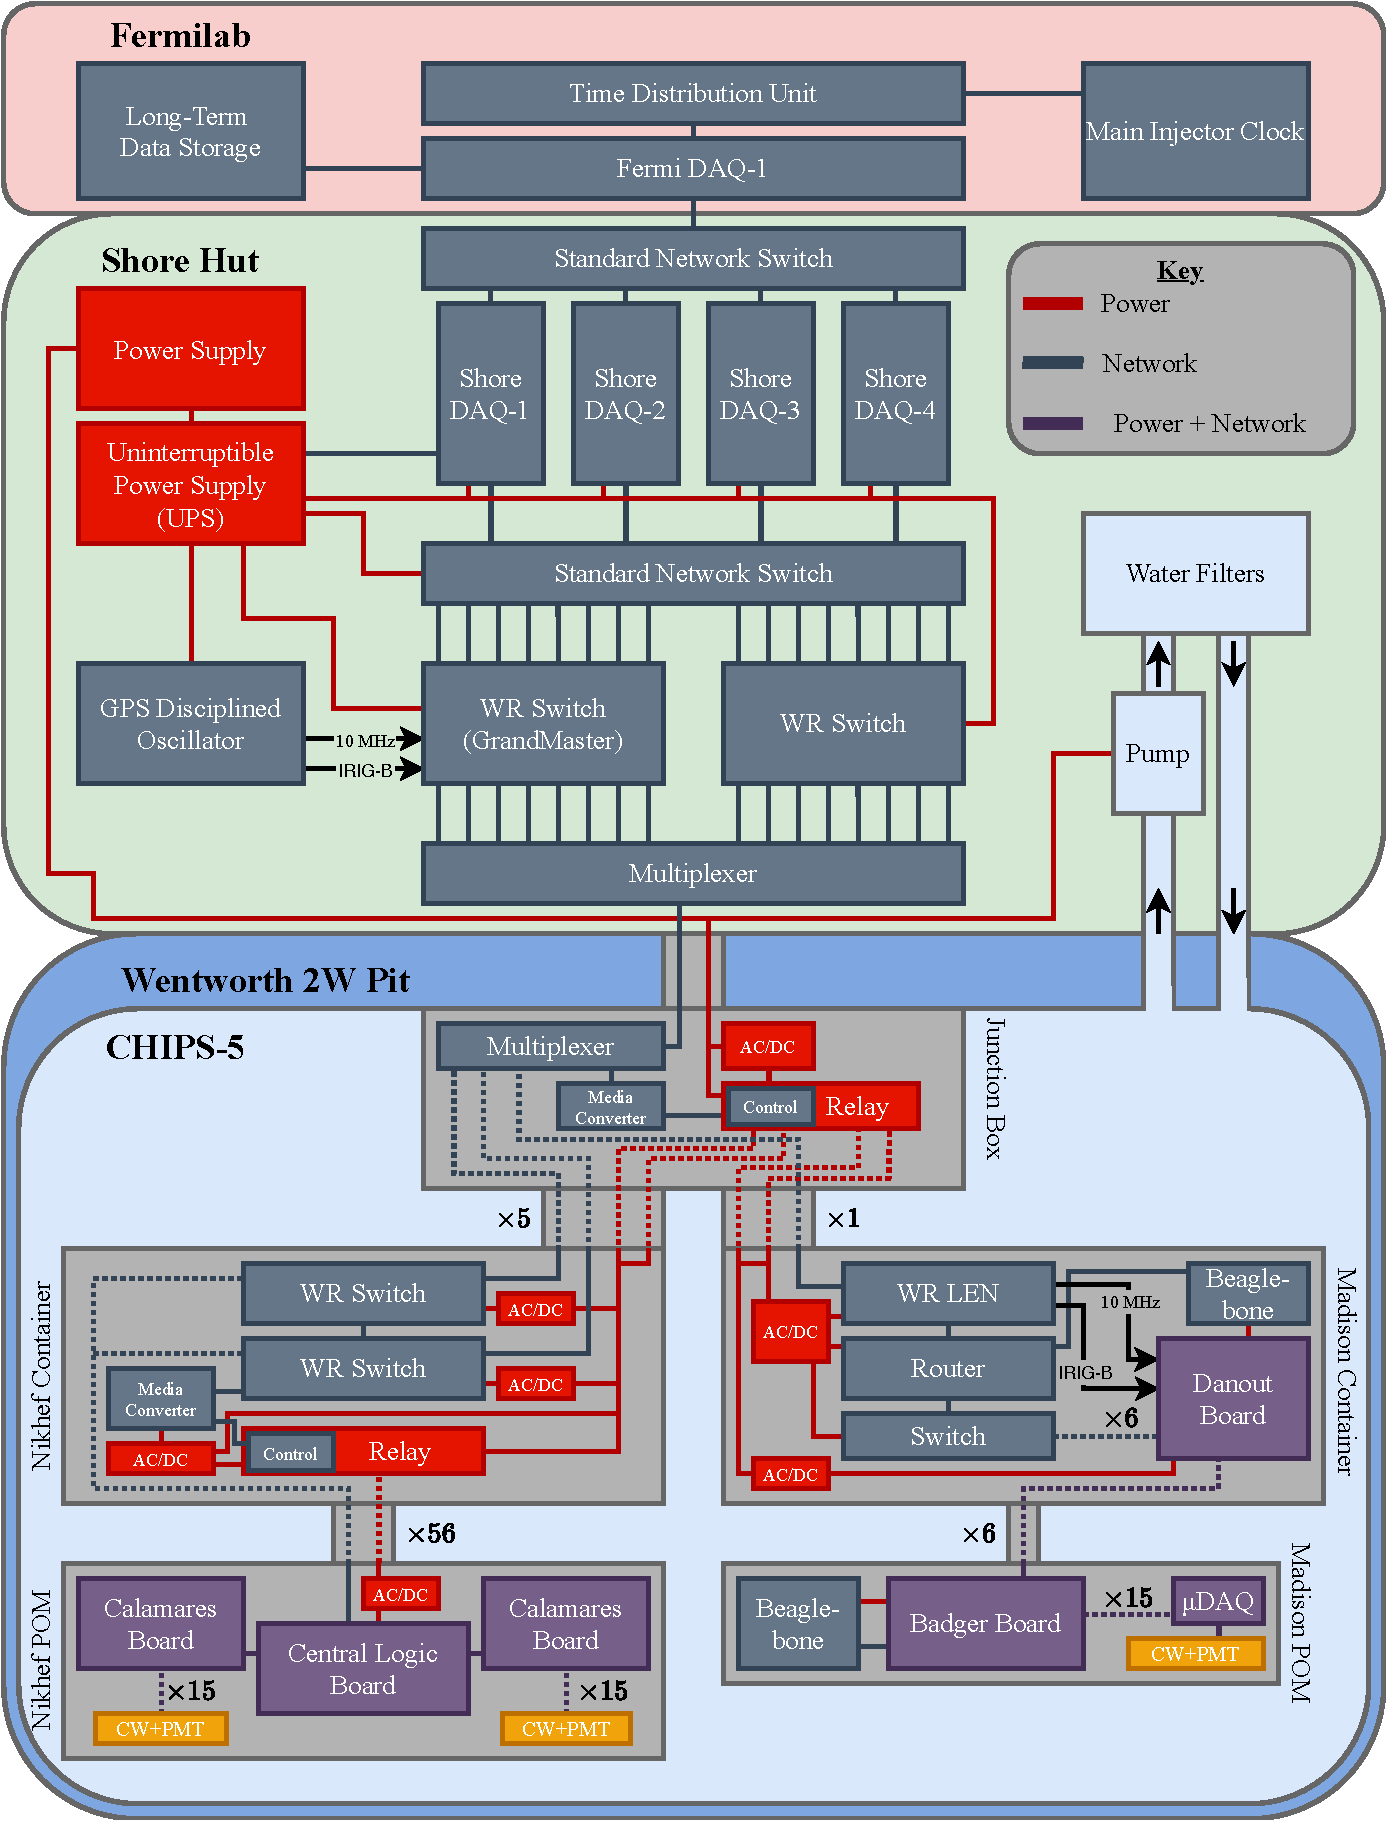
\includegraphics[width=\textwidth]{diagrams/5-daq/daq.pdf}
    \caption[Diagram of the \chipsfive data acquisition and power distribution system.]
    {Diagram of the \chipsfive DAQ and power distribution system.}
    \label{fig:daq}
\end{figure}

\begin{figure} % FULL SETUP DIAGRAM %
    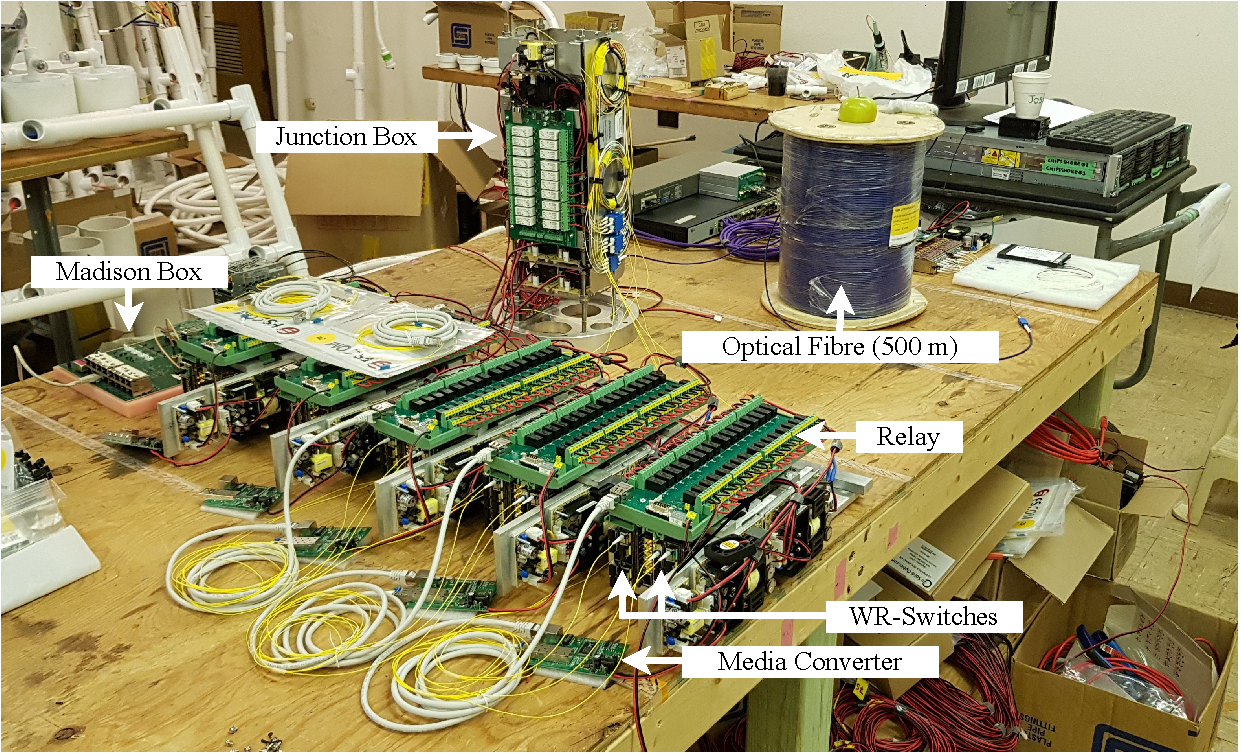
\includegraphics[width=\textwidth]{diagrams/5-daq/full_setup.pdf}
    %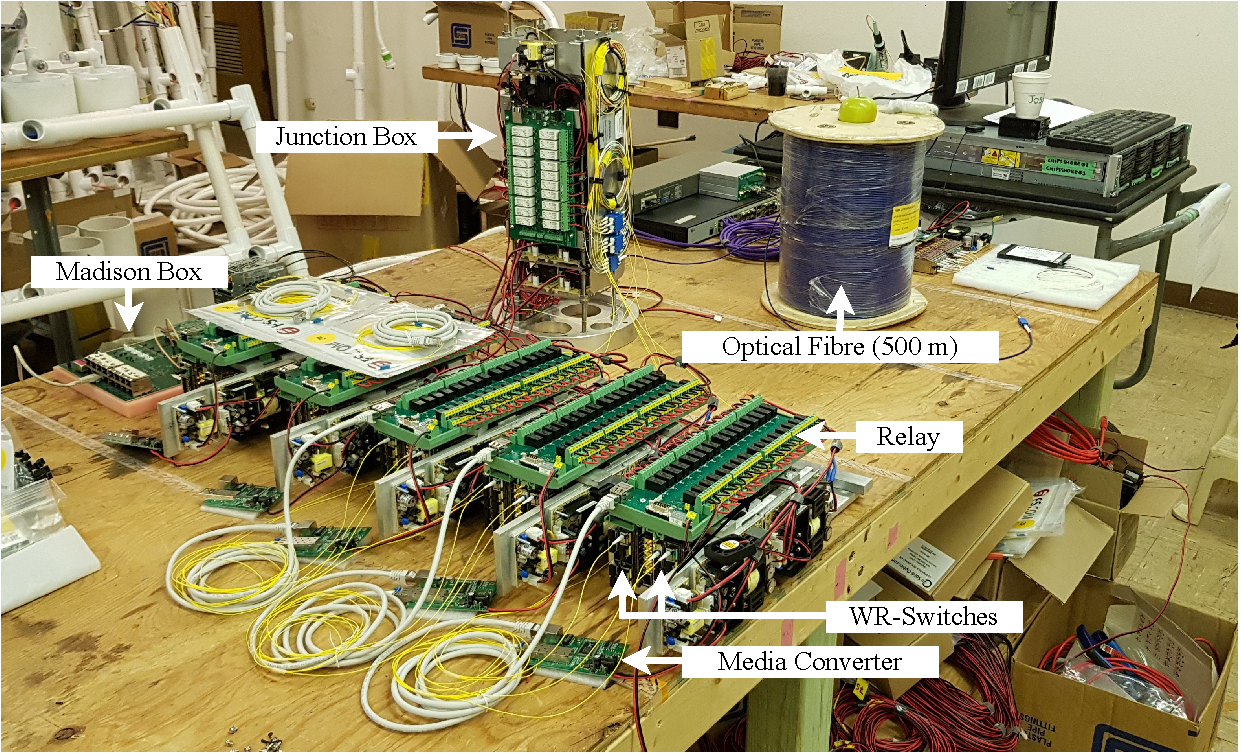
\includegraphics[angle=90,origin=c,width=0.8\textwidth]{diagrams/5-daq/full_setup.pdf}
    \caption[full set up short]
    {Picture of the full \chipsfive DAQ system}
    \label{fig:full_setup}
\end{figure}f

\subsection{Km3NET hardware} %%%%%%%%%%%%%%%%%%%%%%%%%%%%%%%%%%%%%%%%%%%%%%%%%%%%%%%%%%%%%%%%%%%%%
\label{sec:daq_hard_km3net} %%%%%%%%%%%%%%%%%%%%%%%%%%%%%%%%%%%%%%%%%%%%%%%%%%%%%%%%%%%%%%%%%%%%%%

- km3net daq ref in~\cite{biagi2015, adrian2016, eijk2015}

\begin{figure} % NIKHEF PMT AND CLB DIAGRAM %
    \centering
    \subcaptionbox{nikhef pmt\label{fig:nikhef_pmt}}{%
        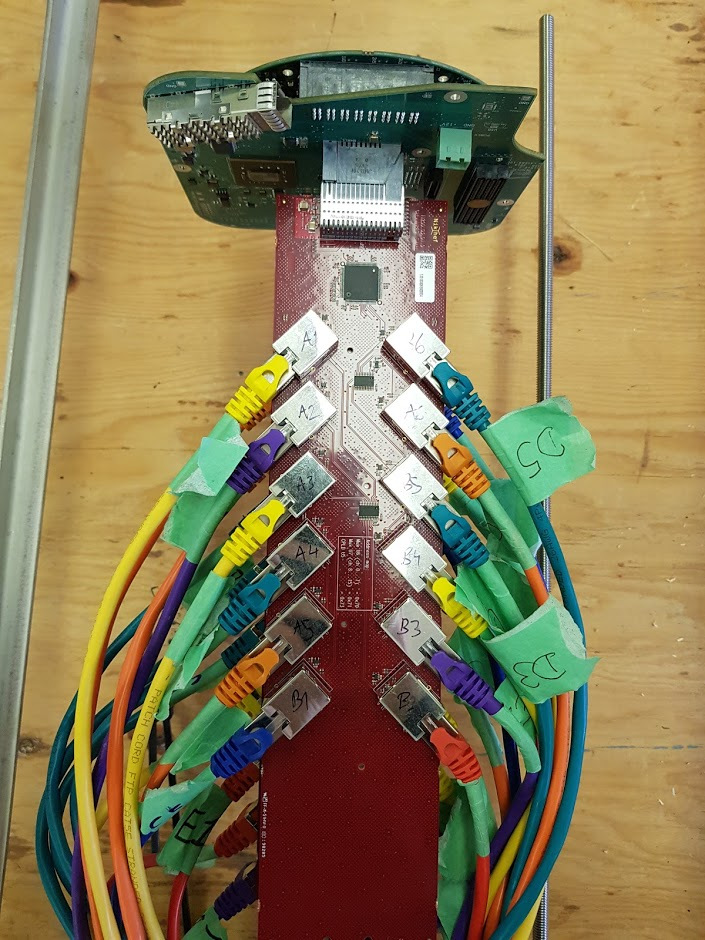
\includegraphics[height=8cm]{diagrams/5-daq/clb.jpg}%
    }
    \quad
    \subcaptionbox{clb\label{fig:clb}}{%
        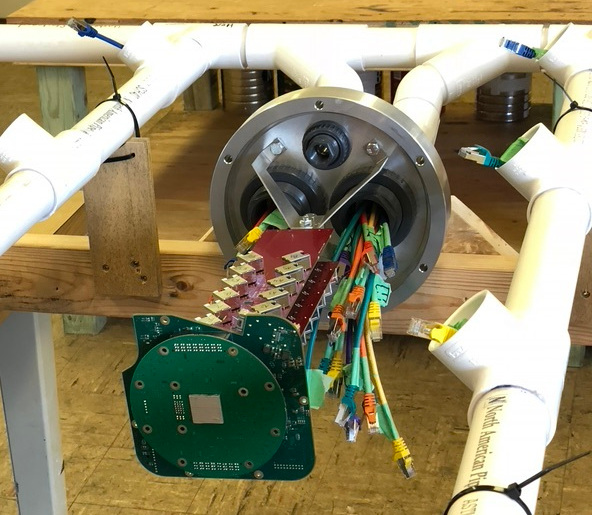
\includegraphics[height=8cm]{diagrams/5-daq/clb_on_plane.jpeg}%
    }
    \caption[The caption]
    {The caption}
\end{figure}

\subsection{Madison hardware} %%%%%%%%%%%%%%%%%%%%%%%%%%%%%%%%%%%%%%%%%%%%%%%%%%%%%%%%%%%%%%%%%%%%
\label{sec:daq_hard_madison} %%%%%%%%%%%%%%%%%%%%%%%%%%%%%%%%%%%%%%%%%%%%%%%%%%%%%%%%%%%%%%%%%%%%%

Daan short ref in~\cite{eijk2018}

\begin{figure} % MADISON BOX DIAGRAM %
    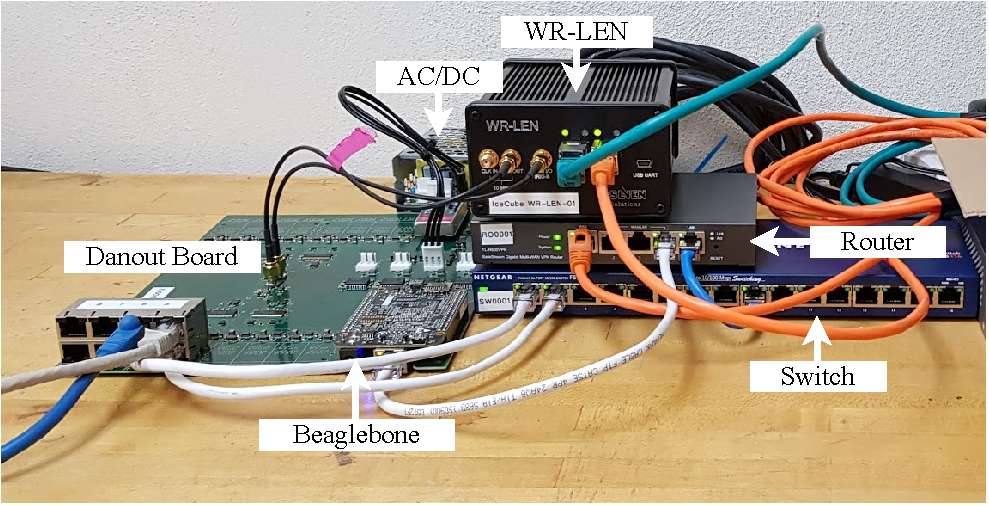
\includegraphics[width=\textwidth]{diagrams/5-daq/madison_box.pdf}
    \caption[madison box short]
    {madison box long}
    \label{fig:madison_box}
\end{figure}

\subsection{Combined systems} %%%%%%%%%%%%%%%%%%%%%%%%%%%%%%%%%%%%%%%%%%%%%%%%%%%%%%%%%%%%%%%%%%%%
\label{sec:daq_hard_combined} %%%%%%%%%%%%%%%%%%%%%%%%%%%%%%%%%%%%%%%%%%%%%%%%%%%%%%%%%%%%%%%%%%%%

\begin{figure} % MANIFOLD DIAGRAM %
    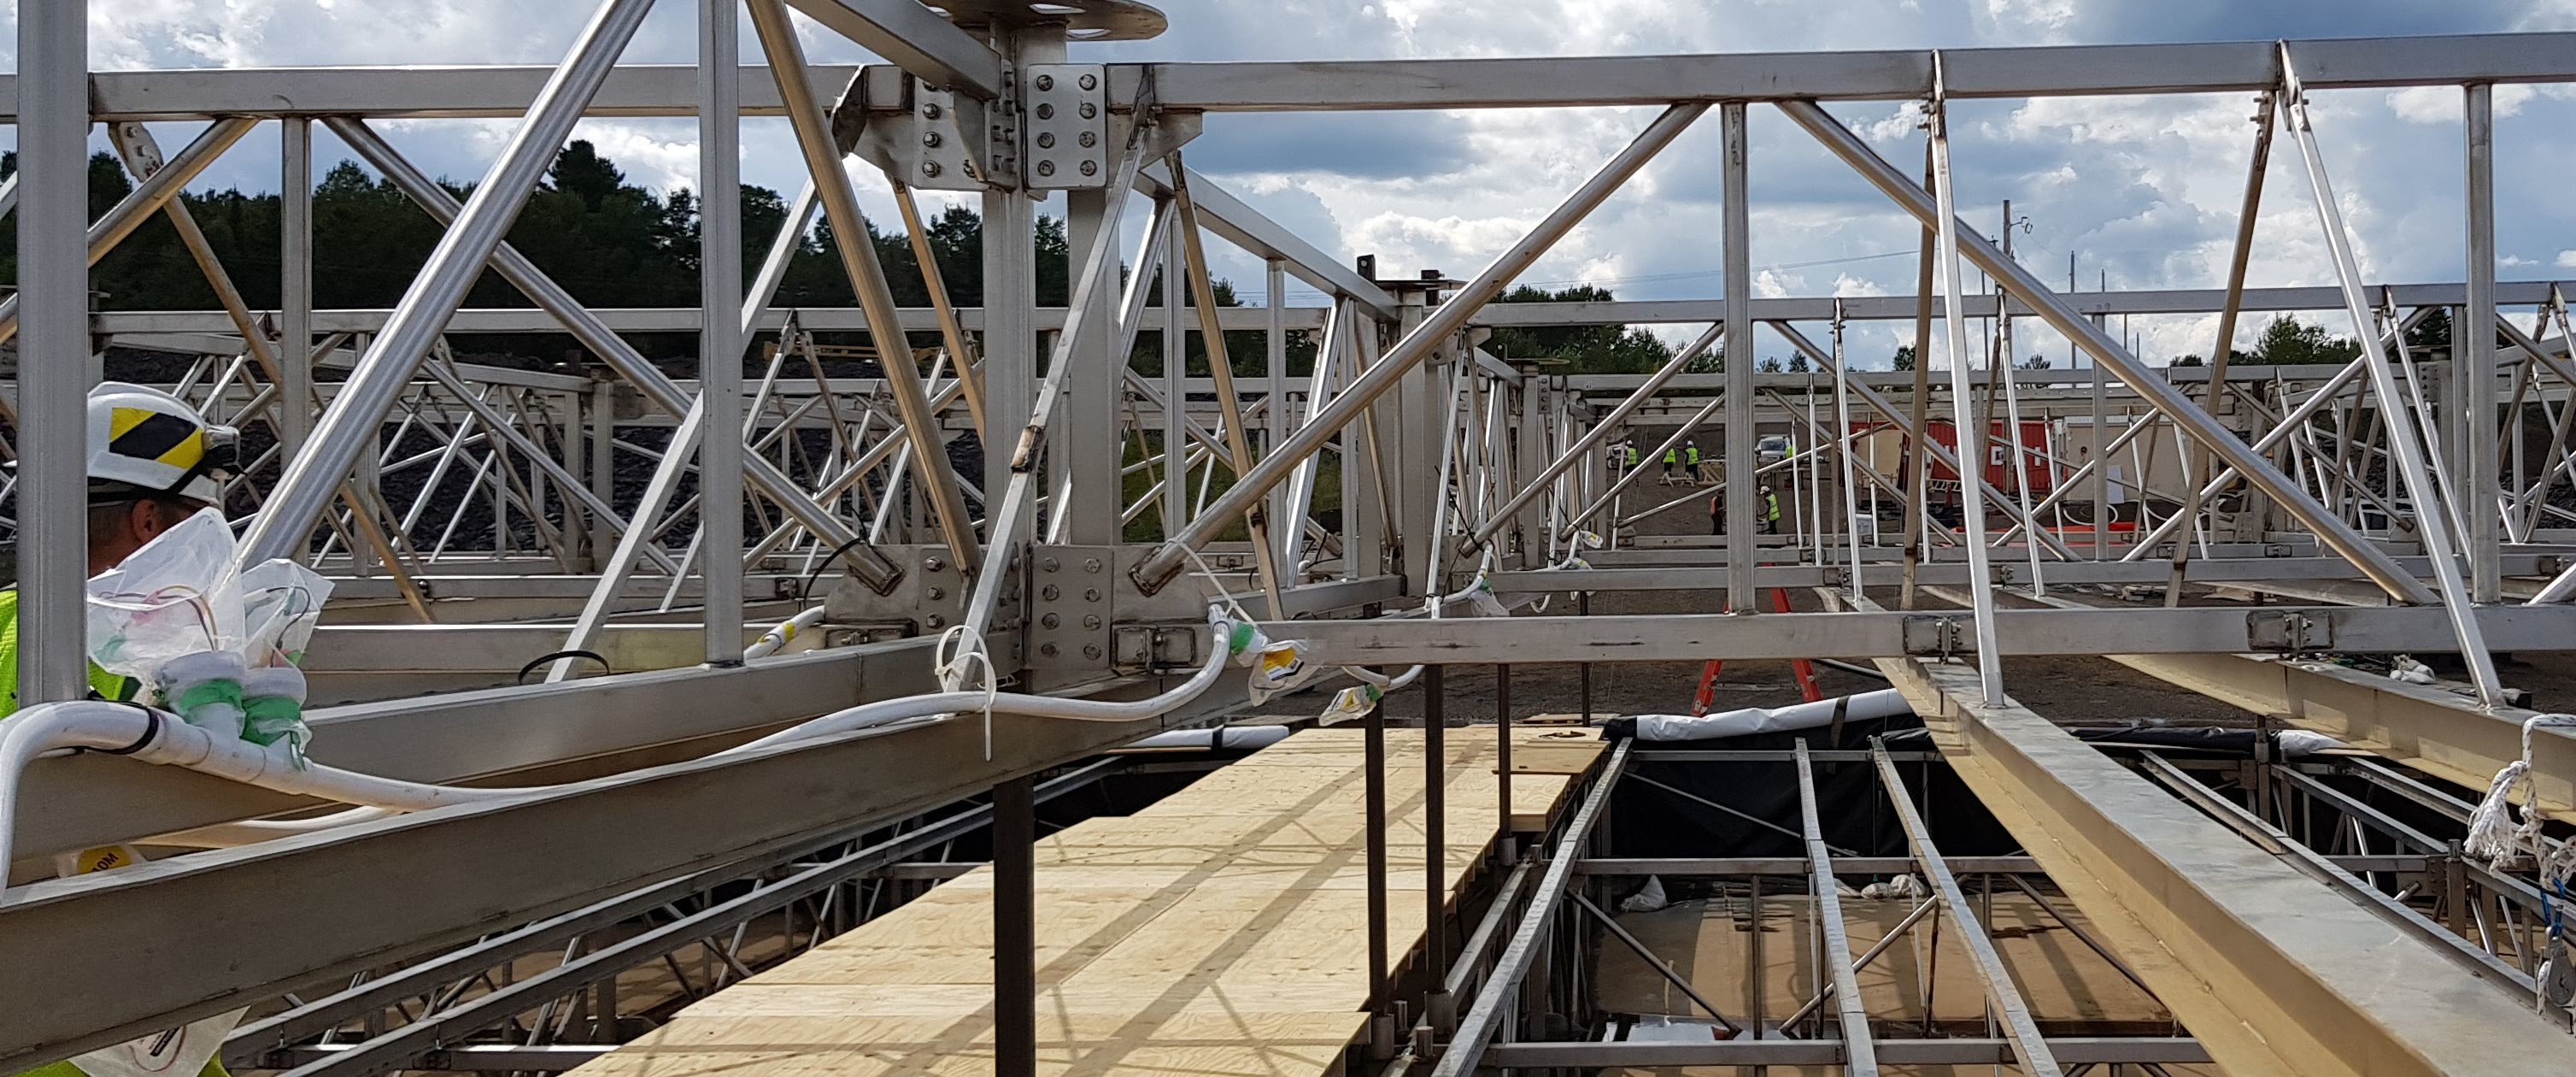
\includegraphics[width=\textwidth]{diagrams/5-daq/manifold.jpg}
    \caption[manifold short]
    {manifold long}
    \label{fig:manifold}
\end{figure}


\begin{figure} % JELLY DIAGRAM %
    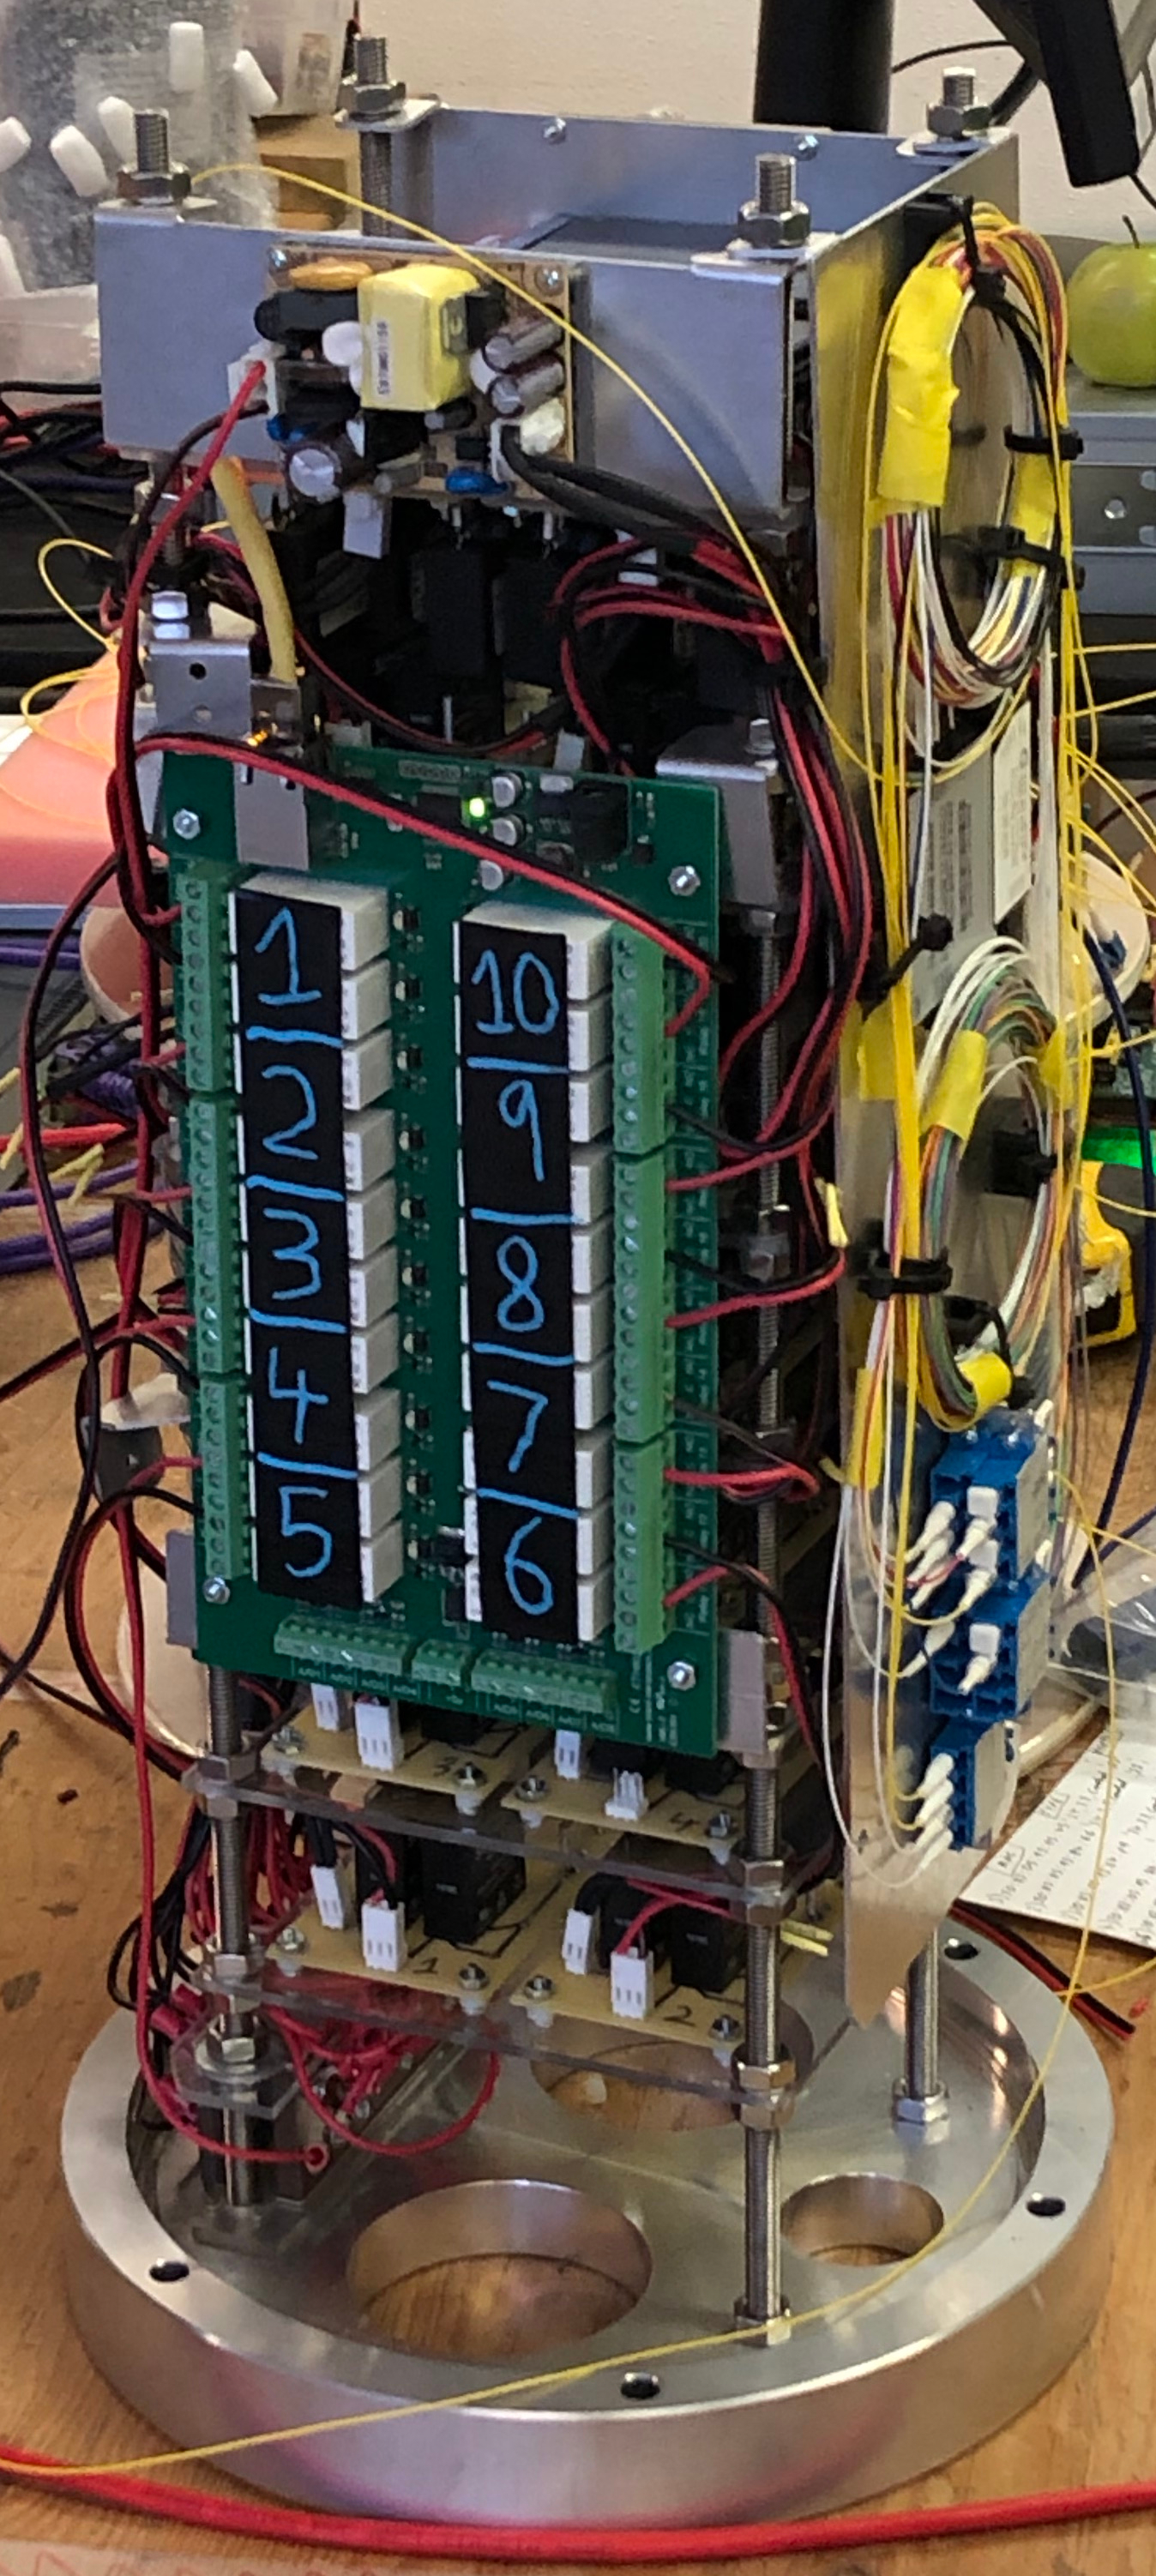
\includegraphics[width=0.5\textwidth]{diagrams/5-daq/jelly.jpeg}
    \caption[jelly short]
    {jelly long}
    \label{fig:jelly}
\end{figure}

\begin{figure} % WHITE-RABBIT GM SETUP DIAGRAM %
    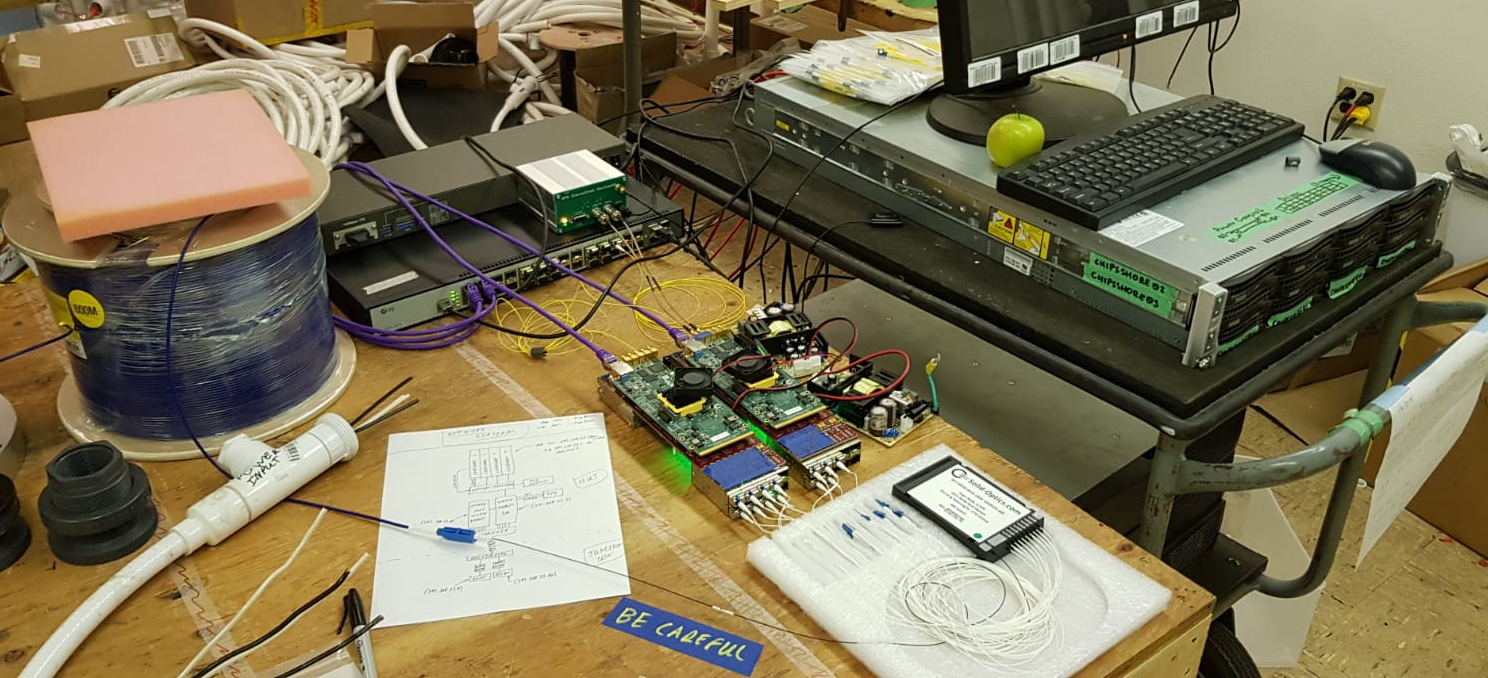
\includegraphics[width=\textwidth]{diagrams/5-daq/hut_daq.jpg}
    \caption[hut daq short]
    {hut daq long}
    \label{fig:hut_daq}
\end{figure}

\section{Software} %%%%%%%%%%%%%%%%%%%%%%%%%%%%%%%%%%%%%%%%%%%%%%%%%%%%%%%%%%%%%%%%%%%%%%%%%%%%%%%
\label{sec:daq_soft} %%%%%%%%%%%%%%%%%%%%%%%%%%%%%%%%%%%%%%%%%%%%%%%%%%%%%%%%%%%%%%%%%%%%%%%%%%%%%

DIAGRAM: Software diagram + finite state machine

\subsection{The beam spill} %%%%%%%%%%%%%%%%%%%%%%%%%%%%%%%%%%%%%%%%%%%%%%%%%%%%%%%%%%%%%%%%%%%%%%
\label{sec:daq_soft_spill} %%%%%%%%%%%%%%%%%%%%%%%%%%%%%%%%%%%%%%%%%%%%%%%%%%%%%%%%%%%%%%%%%%%%%%%

\subsection{Hit acquisition and handling} %%%%%%%%%%%%%%%%%%%%%%%%%%%%%%%%%%%%%%%%%%%%%%%%%%%%%%%%
\label{sec:daq_soft_hits} %%%%%%%%%%%%%%%%%%%%%%%%%%%%%%%%%%%%%%%%%%%%%%%%%%%%%%%%%%%%%%%%%%%%%%%%

\subsection{Detector and data quality monitoring} %%%%%%%%%%%%%%%%%%%%%%%%%%%%%%%%%%%%%%%%%%%%%%%%
\label{sec:daq_soft_monitor} %%%%%%%%%%%%%%%%%%%%%%%%%%%%%%%%%%%%%%%%%%%%%%%%%%%%%%%%%%%%%%%%%%%%%

REF: Elasticsearch paper

\begin{figure} % MONITORING DIAGRAM %
    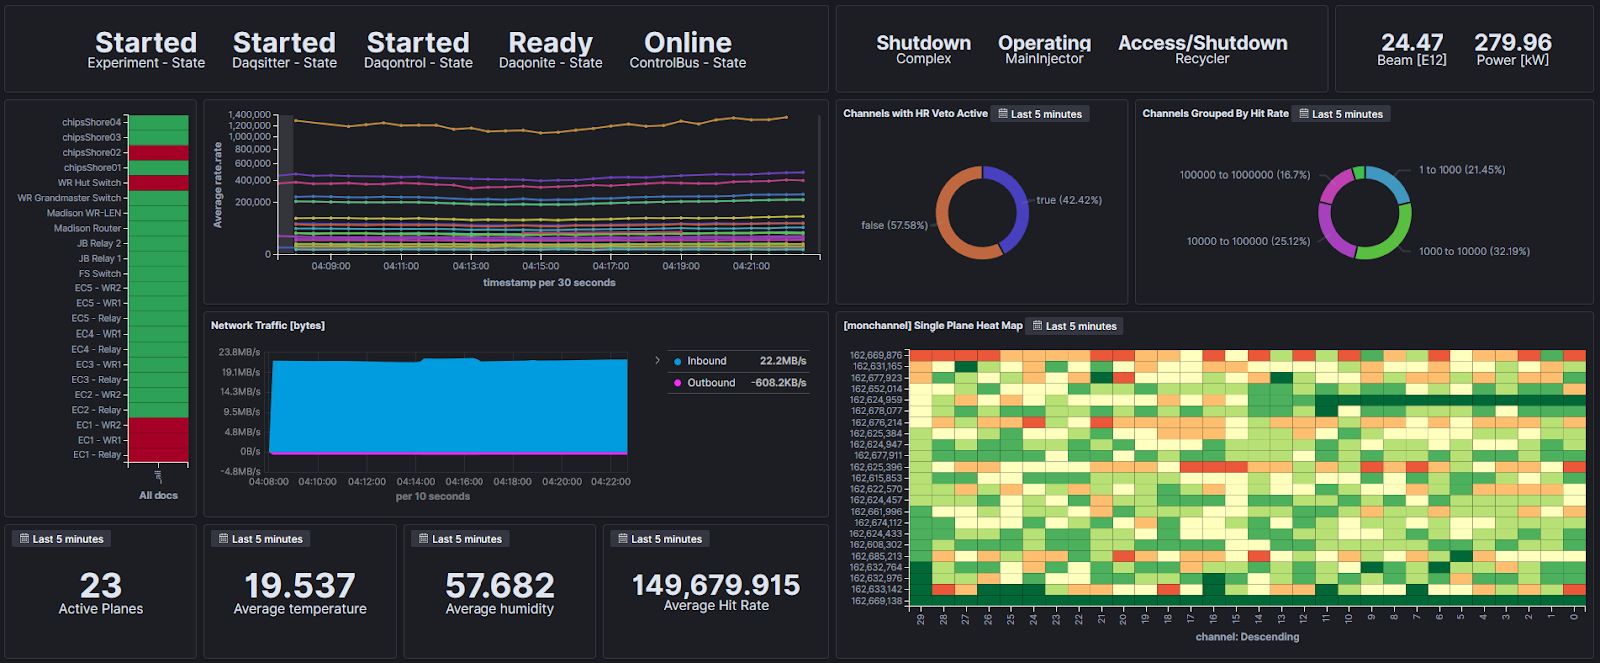
\includegraphics[width=\textwidth]{diagrams/5-daq/monitoring.png}
    \caption[monitoring short]
    {monitoring long}
    \label{fig:monitoring}
\end{figure}